%%%%%%%%%%%%%%%%%%%%%%%%%%%%%%%%%%%%%%%%%%%%%%%%%%%%%%%%%%%%%%%%%%%%%%%%%%%%
% AGUJournalTemplate.tex: this template file is for articles formatted with LaTeX
%
% This file includes commands and instructions
% given in the order necessary to produce a final output that will
% satisfy AGU requirements, including customized APA reference formatting.
%
% You may copy this file and give it your
% article name, and enter your text.
%
%
% Step 1: Set the \documentclass
%
%

%% To submit your paper:
\documentclass[draft]{agujournal2019}
\usepackage{url} %this package should fix any errors with URLs in refs.
\usepackage{lineno}
\usepackage{booktabs}
\usepackage{lscape}
\usepackage[inline]{trackchanges} %for better track changes. finalnew option will compile document with changes incorporated.
\usepackage{textcomp}
\usepackage{mathtools}
\usepackage{soul}
\linenumbers
%%%%%%%
% As of 2018 we recommend use of the TrackChanges package to mark revisions.
% The trackchanges package adds five new LaTeX commands:
%
%  \note[editor]{The note}
%  \annote[editor]{Text to annotate}{The note}
%  \add[editor]{Text to add}
%  \remove[editor]{Text to remove}
%  \change[editor]{Text to remove}{Text to add}
%
% complete documentation is here: http://trackchanges.sourceforge.net/
%%%%%%%

\draftfalse

%% Enter journal name below.
%% Choose from this list of Journals:
%
% JGR: Atmospheres
% JGR: Biogeosciences

% JGR: Earth Surface
% JGR: Oceans
% JGR: Planets
% JGR: Solid Earth
% JGR: Space Physics
% Global Biogeochemical Cycles
% Geophysical Research Letters
% Paleoceanography and Paleoclimatology
% Radio Science
% Reviews of Geophysics
% Tectonics
% Space Weather
% Water Resources Research
% Geochemistry, Geophysics, Geosystems
% Journal of Advances in Modeling Earth Systems (JAMES)
% Earth's Future
% Earth and Space Science
% Geohealth
%
% ie, \journalname{Water Resources Research}

\journalname{JGR: Earth Surface}


\begin{document}

%% ------------------------------------------------------------------------ %%
%  Title
%
% (A title should be specific, informative, and brief. Use
% abbreviations only if they are defined in the abstract. Titles that
% start with general keywords then specific terms are optimized in
% searches)
%
%% ------------------------------------------------------------------------ %%

% Example: \title{This is a test title}

\title{Three-Dimensional Morphometry of Ooids in Oolites}

%% ------------------------------------------------------------------------ %%
%
%  AUTHORS AND AFFILIATIONS
%
%% ------------------------------------------------------------------------ %%

% Authors are individuals who have significantly contributed to the
% research and preparation of the article. Group authors are allowed, if
% each author in the group is separately identified in an appendix.)

% List authors by first name or initial followed by last name and
% separated by commas. Use \affil{} to number affiliations, and
% \thanks{} for author notes.
% Additional author notes should be indicated with \thanks{} (for
% example, for current addresses).

% Example: \authors{A. B. Author\affil{1}\thanks{Current address, Antartica}, B. C. Author\affil{2,3}, and D. E.
% Author\affil{3,4}\thanks{Also funded by Monsanto.}}

\authors{Bolton Howes \affil{1}, Akshay Mehra \affil{1,2}, Adam Maloof \affil{1}}


% \affiliation{1}{First Affiliation}
% \affiliation{2}{Second Affiliation}
% \affiliation{3}{Third Affiliation}
% \affiliation{4}{Fourth Affiliation}

\affiliation{1}{Department of Geosciences, Princeton University, Guyot Hall, Washington Road, Princeton, NJ 08544, USA }
\affiliation{2}{Department of Earth Sciences, Dartmouth College, Hanover, NH, 03755, USA }


%(repeat as many times as is necessary)

%% Corresponding Author:
% Corresponding author mailing address and e-mail address:

% (include name and email addresses of the corresponding author.  More
% than one corresponding author is allowed in this LaTeX file and for
% publication; but only one corresponding author is allowed in our
% editorial system.)

% Example: \correspondingauthor{First and Last Name}{email@address.edu}

\correspondingauthor{Bolton Howes}{bhowes@princeton.edu}

%% Keypoints, final entry on title page.

%  List up to three key points (at least one is required)
%  Key Points summarize the main points and conclusions of the article
%  Each must be 100 characters or less with no special characters or punctuation and must be complete sentences

% Example:
% \begin{keypoints}
% \item	List up to three key points (at least one is required)
% \item	Key Points summarize the main points and conclusions of the article
% \item	Each must be 100 characters or less with no special characters or punctuation and must be complete sentences
% \end{keypoints}

%\begin{keypoints}
%\item enter point 1 here
%\item enter point 2 here
%\item enter point 3 here
%\end{keypoints}

%% ------------------------------------------------------------------------ %%
%
%  ABSTRACT and PLAIN LANGUAGE SUMMARY
%
% A good Abstract will begin with a short description of the problem
% being addressed, briefly describe the new data or analyses, then
% briefly states the main conclusion(s) and how they are supported and
% uncertainties.

% The Plain Language Summary should be written for a broad audience,
% including journalists and the science-interested public, that will not have 
% a background in your field.
%
% A Plain Language Summary is required in GRL, JGR: Planets, JGR: Biogeosciences,
% JGR: Oceans, G-Cubed, Reviews of Geophysics, and JAMES.
% see http://sharingscience.agu.org/creating-plain-language-summary/)
%
%% ------------------------------------------------------------------------ %%

%% \begin{abstract} starts the second page

\begin{abstract}
The prevalence of ooids in the stratigraphic record and their well-established association with shallow-water carbonate environments make ooids an important paleoenvironmental indicator. Studies of modern ooids in  Turks and Caicos and The Bahamas have demonstrated that the size and shape of ooids depend on the depositional environment and peak water velocity. These findings suggest that we can leverage the morphology of ooids in ancient oolites as indicators of depositional environment and paleohydraulic conditions. Currently, researchers measure the size and shape of lithified ooids on two-dimensional surfaces (i.e. thin sections or polished slabs), which often requires researchers to assume the random 2D slice intersects the center of the ooid, and that the ooid is spherical. Here we demonstrate that this assumption is rarely true, and results in errors of up to 35\% on measurements as simple as major axis length. Accurate measurement of the size and shape of ooids in a lithified sample requires that the measurements be made on three dimensional reconstructions. We present a method for making 3D reconstructions by serial grinding and image processing. Our method accurately measures the size (axes lengths, volume, and surface area), shape (prolateness and oblateness), and growth history of individual ooids within an oolite, as well as the sorting and porosity of the sample. The ability to extract these measurements from an oolite means we can use the relationship between ooid morphology, depositional setting, and hydraulic conditions determined from studies of modern carbonate platforms as a tool for understanding ancient carbonate environments.
\end{abstract}

%\section*{Plain Language Summary}

%%% Suggested section heads:
% \section{Introduction}
%
% The main text should start with an introduction. Except for short
% manuscripts (such as comments and replies), the text should be divided
% into sections, each with its own heading.

% Headings should be sentence fragments and do not begin with a
% lowercase letter or number. Examples of good headings are:

% \section{Materials and Methods}
% Here is text on Materials and Methods.
%
% \subsection{A descriptive heading about methods}
% More about Methods.
%
% \section{Data} (Or section title might be a descriptive heading about data)
%
% \section{Results} (Or section title might be a descriptive heading about the
% results)
%
% \section{Conclusions}


\section{Introduction}
%Text here ===>>>
Ooids are concentrically-laminated carbonate grains that are abundant in shallow-water carbonate environments spanning the Archean to the Modern. The prevalence of ooids in shallow-water carbonate rocks, and the narrow depth range of their formation \cite{Geyman2018,harris2019formation}, make ooids a particularly valuable paleoenvironmental proxy and a stable frame of reference for comparing carbonate platforms throughout Earth's history. Carbonate platforms contain a mosaic of subenvironments (facies) like oolitic shoals, beaches, lagoons, tidal channels, etc. Each of these environments has unique chemical and physical conditions, which produce ooids with facies-dependent sizes and shapes (Figure \ref{fig:equil_size}a\&b;  \citeA{mariotti2018contribution}; \citeA{trower2018active}). Consequently, the morphology of ooids and their lamellae can be used to refine facies models of ancient carbonate platforms and improve paleoenvironmental reconstructions. 

 While some features of ooid growth remain mysterious, there is general agreement that ooids grow from the precipitation of calcium carbonate onto the surface of a suspended nucleus or an existing ooid \cite{bathurst1972carbonate}. The ooid continues to grow until it is either buried, too big to be transported \cite{sumner1993numerical}, or precipitation and abrasion rates reach a dynamic equilibrium (Figure \ref{fig:equil_size}c; \citeA{trower2017experimental}). This model provides a useful heuristic for understanding the relationship between environmental conditions and ooid size by indicating that increased precipitation rates and more frequent ooid transport lead to larger ooids.

Like size,  the shape of the ooid reflects the conditions under which the ooid formed. The shape of an ooid is the product of collisions during saltation and friction with the substrate, which produce spherical and flattened shapes respectively \cite{domokos2012evolution,sipos2018shape}. Based on the shape evolution model of ooids described by \citeA{sipos2018shape}, spherical ooids should become elongated if the primary transport mode changes from saltation to bed-load transport. An ooid's lamellae preserve the history of an ooid's shape as it grows. This growth history may contain information about how sediment transport changes as the grain size---and mass---increases \cite{heller1980transport}. Understanding how transport mode changes as a function of size can provide clues about paleohydraulic conditions of ooid-forming environments and perhaps elucidate the formation of giant ooids, which must have formed under uniquely saturated and/or turbulent conditions to reach their size \cite{heller1980transport,sumner1993numerical,sipos2018shape, trower2020enigma}.

Lithified ooids typically have the same composition and physical properties as the binding cement, precluding measurement through physical separation or x-ray computed tomographic techniques. The inability to make 3D measurements has forced researchers to measure the size and shapes of ooids on polished surfaces and in thin sections. Previous research has demonstrated that it is not possible to accurately characterize 3D size and shape distributions from 2D measurements \cite{dehoff1983quantitative,mehra2018multiscale}. We expand on those results by presenting synthetic experiments with spherical and ellipsoidal shapes, demonstrating that estimates of 3D morphology from measurements made on a 2D cross section can be highly inaccurate (Figure \ref{fig:sphere_error}). To overcome the limitations of 2D measurements, we serially ground, imaged, and segmented oolites using the Grinding, Imaging, and Reconstruction Instrument (GIRI) at Princeton University \cite{mehra2018multiscale}, resulting in quantitative 3D reconstruction that enable accurate measurement of ooid size and shape. 

\begin{figure}[h]
    \centering
    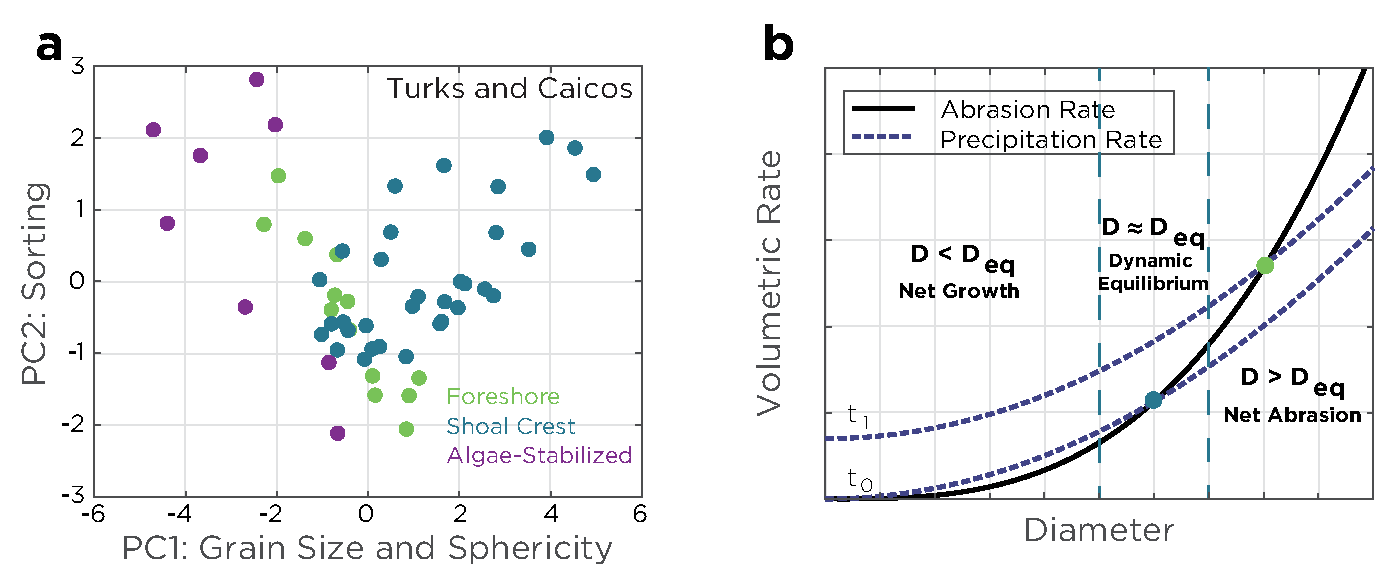
\includegraphics[width = 1\textwidth]{equilib_pcafig.eps}
    \caption{
    (a) Principal component analysis (PCA) of the size and shape of modern ooids from the Turks and Caicos demonstrates that the morphometry of ooids is facies dependent \citeA{trower2017experimental}. (b) Carbonate saturation state and the hydraulic conditions determine the size of an ooid. For example, if the precipitation rate increases (as seen in the upward shift from \(t_0\) to \(t_1\)), the precipitation rate also will increase and the ooid will reach a new equilibrium size (light green dot). Modified from \citeA{trower2017experimental}.} 
    \label{fig:equil_size}
\end{figure}



\section{The necessity of 3D Measurements}

The limitation measurements from thin sections and polished slabs is that these measurements represent 2D apparent dimensions instead of 3D grain dimensions. The two central problems with making 2D measurements on 3D objects are the cut-section effect, which arises because a grain is seldom cut exactly through its center, and the intersection probability effect, because a 2D slice is more likely to intersect a large grain than a small one \cite{higgins2000measurement}. These problems can be partially addressed by applying stereological corrections to the 2D slices \cite{peterson1996refined,sahagian19983d,higgins2000measurement}, but these solutions require assumptions about several parameters of the sample including the size distribution type (e.g. log-normal), particle shape, and sorting of the rock. In the case of ooids in an oolite, shape and sorting are parameters we need to know in order to deduce environment (Figure \ref{fig:equil_size}a\&b), so we cannot make these assumptions. Furthermore, these assumptions may not be valid for ooids. For example, ooids within the same layer can be many different shapes, so assuming a single particle shape for stereological analysis would be inappropriate. Here we quantify the errors associated with 2D measurements, and then present a method for directly measuring the size and shape distribution of ooids in an oolite from a 3D reconstruction.

\subsection{Size Errors in 2D}
Even simple size distributions of spherical and ellipsoidal grains are difficult, if not impossible, to accurately describee from 2D measurements. The measurement of the diameter of a population of grains with a normally-distributed major axis length shows that the 2D apparent size underestimates the true size distribution (Figure \ref{fig:sphere_error}a\&b). For spheres in this experiment, the error is solely due to the cut-section effect. In ellipsoids, the error associated with 2D measurements arises from the cut-section effect as well as intersections that are nearly perpendicular to the major axis mistaking the major and intermediate axes (Figure \ref{fig:sphere_error}c). Similarly, attempts to measure the intermediate axis are complicated by both the cut-section effect and mistaking the minor axis for the intermediate axis when the intersection is nearly perpendicular to the intermediate axis (Figure \ref{fig:sphere_error}d). Error from 2D measurements of the major axis of an ellipsoid increases as the ellipsoid becomes less spherical, especially as the ellipsoid becomes more prolate (Figure \ref{fig:sphere_error}e), reaching 35\% when the major axis is twice as long as the intermediate axis. For ooids with an aspect ratio similar to those from Turks and Caicos \cite{trower2018active}, we expect errors of ~15\%, which means 85\% of the samples would have indistinguishable D50 values (50th percentile of grain diameters). This error would preclude identification of depositional environments based on ooid shape and size because it is the most heavily weighted variabel in PC1 from the PCA in Figure \ref{fig:equil_size}. In an attempt to overcome the cut-section effect, it is common practice for researchers to measure only ooids they believe are cut through the nucleus, but we demonstrate that while this technique is better, there are still errors of up to 30\% depending on the size of the nucleus and the shape of the ooid (Figure \ref{fig:sphere_error}f), not to mention the difficulty in identifying an ooid's nucleus (Figure \ref{fig:grown_flattening}a--d). The reader should note that these experiments only account for the cut-section effect, so they can be considered minimum-error scenarios. 


\subsection{Shape Errors in 2D}
Just as with size, 2D apparent dimensions provide inaccurate approximations of 3D shape. For example, we consider a single synthetic ooid with five growth lamellae and measure the prolateness of the ellipsoid represented by each lamellae with 2500 random intersections of the ooid (Figure \ref{fig:grown_flattening}d). Even if we only include the planes that intersect all five growth bands, the resulting estimate of prolateness (intermediate axis length divided by long axis length) for a single lamination varies by up to 30\%, and the percent error of the median measurement is wrong by up to 13.9\% (\ref{fig:grown_flattening}e; this error strongly depends on the shape of the growth band as in Figure \ref{fig:sphere_error}e\&d). The random cuts also demonstrate that when an ooid has well-preserved lamellae, it is difficult to determine when a plane truly cuts through the nucleus, which is consistent with natural samples (Figure \ref{fig:grown_flattening}a--d). In Figure \ref{fig:grown_flattening}d, all of the random slices appear to intersect a nucleus, but only because they are synthetic and with a known number of lamellae can we determine which are cut through the nucleus. Additionally, some ooids have obvious nuclei (like a shell or fragment of another ooid), but these nuclei can have irregular or elongated shapes and there will be substantial error from missing the center of the nucleus (Figure \ref{fig:AR_Growth}c). Combined, these problems with 2D measurements of ooid lamellae demonstrate that studies of ooid shape and growth history require 3D reconstructions.   


\subsection{Porosity Errors in 2D}
Accurate porosity estimates are crucial for understanding the potential of a rock for both oil extraction and CO\(_2\) sequestration, as well as modeling interstitial fluid flow. Just as 2D sections are unreliable recorders of size and shape (Figure \ref{fig:sphere_error}), individual 2D sections are also unable to accurately describe porosity. For instance, when estimating porosity by measuring the area of every grain and void space on 1000 random sections through an oolite, any one estimate can be up to 30\% wrong (Figure \ref{fig:porosity_error}a). Error will increase when measuring only a subset of grains on each sample (e.g., via point counting). Additionally, while an average of multiple sections can approximate volumetric porosity, a large number of measurements are required to achieve high accuracy: in the synthetic example, it takes 77 fully segmented slices to be withing 5\% of the true porosity value for the volume, and 273 slices to be within 1\% of the true value (Figure \ref{fig:porosity_error}b).     

\section{Materials and Methods}
\subsection{Making 3D Measurements}
To make direct measurements in 3D, we serially ground and imaged an oolite collected from Joulter's Cay, Andros Island, The Bahamas. The sample is a lightly-cemented oolite associated with aeolian coastal dunes formed near an active oolitic shoreface \cite{halley1979fresh}. There are 30 \(\mu\)m between images, and the pixel size in each image is 5.6 \(\mu m\). For complete details of the grinding and imaging routine see \citeA{mehra2018multiscale}. The sample contains 847 slices and over 30,000 ooids, each individually segmented and measured via an image processing pipeline.



\begin{figure}
    \centering
    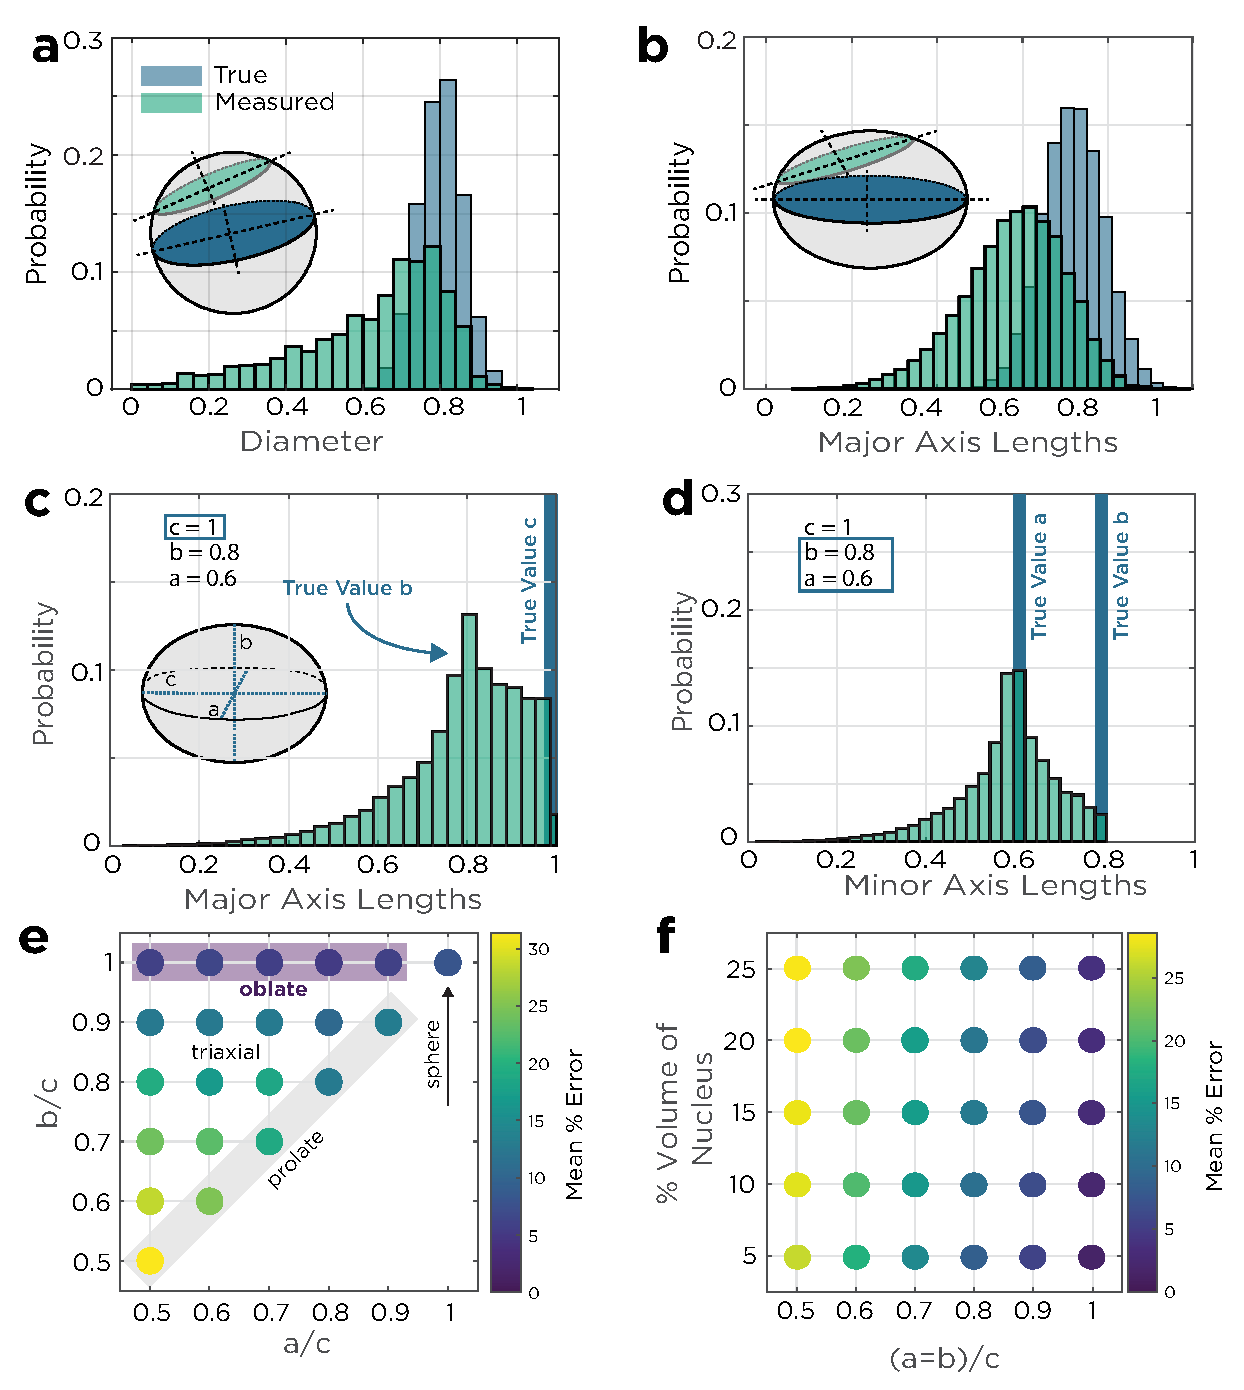
\includegraphics[width = 1\textwidth]{ellipsoid_error_f.eps}
    \caption{(a) The difference between the diameter of a population of spheres and the major axis length measured on cut spheres from the same population demonstrates that 2D cuts of a sphere underestimate the true size distribution of the population. (b) The difference between the true major axis length of population of ellipsoids (a/c = 0.6, b/c = 0.8) and the major axis lengths measured on a random cut through ellipsoids from this distribution. (c) Measurement of the major axis,\textit{c}, of a single ellipsoid on a random 2D slices underestimates the major axis length. (d) Measurement of the minor axis of the ellipse formed by a random intersection with an ellipsoid leads to error in the estimation of the minor axes. (e) Each dot represents the mean percent error of the median of 100 measurements of the major axis length for a range of ellipsoid shapes. The mean error increases as the ellipsoids become less spherical and more prolate. (f) Mean percent error of the median of 100 measurements of the long axis on a plane that intersects the nucleus as a function of prolateness and the size of the nucleus. Error increases as the size of the nucleus increases and as grain becomes less spherical.}
    \label{fig:sphere_error}
\end{figure}

\begin{figure}
    \centering
    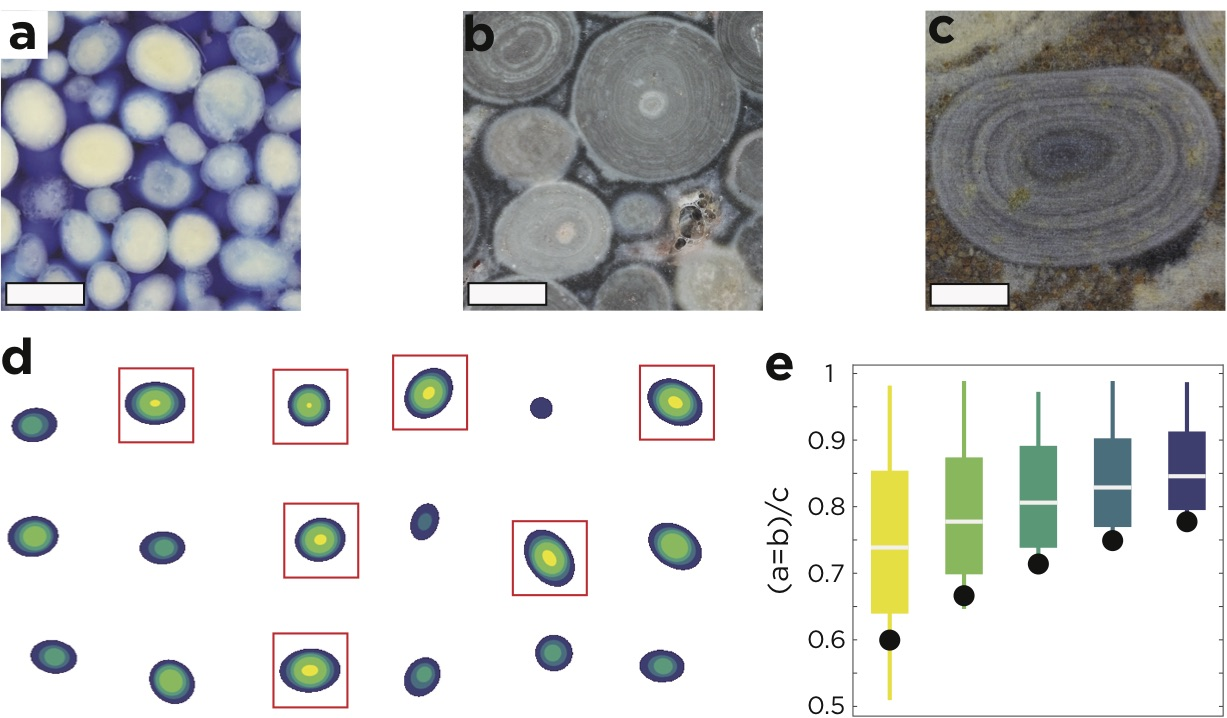
\includegraphics[width = 1\textwidth]{grown_flattening_f.eps}
    \caption{(a) Holocene oolite from Joulter's Cay, The Bahamas. White scale bar is 100 $\mu$m \cite{maclennan2018arc}. (b) Giant ooids from the Tonian Matheos Formation of Ethiopia. White scale bar is 0.5 cm. (c) Giant ooids from the Etina Formation in Australia. White scale bar is 0.5 cm \cite{rose2013end}. (a--c) These photographs demonstrate the difficulty of identifying the nucleus of an ooid from a 2D slice through an oolite. In (a), there are no clear nuclei in any of the ooids, In (b) and (c), banding of the ooids make it appear as if the cut is through the nucleus even though our 3D models reveal that none of the ooids present are actually cut through their nucleus in these slices. (d) 12 of the 2500 random cuts through a synthetic ellipsoidal ooid with five lamellae show the many different cross sections that can be produced from slicing a single ellipsoid. The red boxes outline slices that intersect all five lamellae. (e) The box plot shows the distribution of apparent prolateness values produced from 2D slices of the ooid in (d), and only slices that intersect the nucleus are used to calculate these distributions. From left to right in (e), the error of the median is  13.9\%, 11.1\%, 9.2\%, 7.2\%, and 6.8\%. Two-dimensional slices overestimate how spherical the ooids are because many slices are oblique or perpendicular to the c-axis producing more circular cross-sections. The colors of the box plots match the colors of the lamellae in (d). Black dots mark the true flattening value for the lamellae.}
    \label{fig:grown_flattening}
\end{figure}



\subsection{Image Processing}
Segmenting and measuring of 3D granular particles is a challenging task and an active field of research in computer vision, material sciences, and biology \cite{jaquet2013estimation}. The difficulty arises from needing to separate objects of the same material with a high degree of connectivity---or that have grown together like ooids cemented by calcium carbonate. The first step is to identify all the ooid and non-ooid pixels in an image, for which we used a convolutional neural network (CNN). Using the tracing tools in Dragonfly ORS \cite{DragonflyORS}, we built a training dataset by tracing over  1.25 million pixels of the ooid and 500,000 of the non-ooid class out of a dataset of {\raise.17ex\hbox{$\scriptstyle\sim$}}2 billion pixels (Figure \ref{fig:seg_routine}b). These training pixels are on ten different images distributed throughout the image stack. We then used these training data to train a CNN, which labelled every pixel as either ooid or not ooid (Figure \ref{fig:seg_routine}c). Isolating individual ooids for measurement required implementing a watershed, which consists of finding the distance of every ooid-labelled pixel to the nearest non-ooid labelled pixel (Figure \ref{fig:seg_routine}d), using the regional maximum distance as the ``seeds" for the watershed (Figure \ref{fig:seg_routine}e). Morphological measurements use the Euclidean distance between neighbor voxels and the center structuring element, so we transformed the initial 5.6 x 5.6 x 30 \(\mu m\) voxels to 10 x 10 x 10 \(\mu m\) voxels to remove anisotropy from the dataset. This technique is common practice in 3D imaging techniques like x-ray computed tomography \cite{pierret20023d, capowiez2003characterisation}.  Complete MATLAB code for the CNN and the specifications for the watershed in Avizo (a scientific visualization software package) are provided in the supplement.

\begin{figure}
    \centering
    \includegraphics[width = 1\textwidth]{porosity_error.eps}
    \caption{(a) Measurement of porosity in an oolite based on 2D intersections leads to a distribution of porosity estimates (purple represents a perfectly-packed volume of grains with a log-normal distribution; green is the same as purple, but with randomly added void space throughout the volume). (b) Convergence on the accurate estimate requires the measurement of tens to hundreds of fully-segmented slices.  }
    \label{fig:porosity_error}
\end{figure}


\subsection{Measurements}
Ooid size measurements were made individually on each ooid in MATLAB using the built in \texttt{regionprops3} function, which provides measurements of the principal axis lengths, volume, and surface area. From these measurements it is possible to derive shape and sorting metrics. All particles with a long axis length shorter than 100 \(\mu m\) or longer than 750 \(\mu m\) were removed to filter out non-ooid particles like shells and grapestones. In total, this process takes 5--6 days per sample: 3--4 days to grind and image, 3--4 hours to make a training dataset, then train the neural network and segment the images overnight, then a day for any necessary post-processing. The grinding and imaging is completely automated \cite{mehra2018multiscale}, and the training and post-processing can be optimized when there are multiple samples with similar colors and textures because you can reuse the segmentation model and post-processing routines. 

% It is again worth noting that these size and shape measurements are different from traditional particle size analyzers and camsizers. The measurements presented here are directly made on each grain, whereas particle size analyzers report the distribution of grain sizes in a sample based on the laser diffraction pattern and camsizers measure a projection of the particle. 




\subsection{Joulter's Cay Measurements}
Analysis of the ooids in the Joulter's Cay image stack demonstrates the image processing routine can provide measurements of individual ooids in a lithified oolite (Figure \ref{fig:2D_Hist}a). Since the ooids in the lithified oolite were sourced from the nearby shoreface; we can compare the size of the ooids from the image processing routine to modern ooids collected from the Joulter's Cay shoreface measured with a camsizer and see that they are similar (Figure \ref{fig:2D_Hist}b). We expect the lithified eolianite to show improved sorting over the source shoreface, which is observed: the Joulter's Cay sample has a sorting of 0.70, which is better sorted than any of the 22 ooid samples from a 1 km transect of the nearby shoreface, and is 48\% better than the average shoreface ooid sample on the northern part of Andros Island (sorting is measured using a normalized dispersion parameter, \(\sigma^{\star} = \frac{d5ƒ0 - d90}{d50}\)). Additionally, the error in size estimate would be approximately 20\% for ooids with the a/c and b/c ratio of those in the Joulter's Cay sample based on the simulations in Figure \ref{fig:sphere_error}f. This lack of accuracy and precision in size estimates from 2D measurements along with errors from the intersection probability effect, would have prevented differentiating between eolian and submarine environments without the three-dimensional reconstruction. Additionally, with the fully-segmented image stack we are able to measure the porosity of the oolite: 59.6\% (Figure \ref{fig:2D_Hist}c--d).  



\begin{figure}
    \centering
    \includegraphics[width = 1\textwidth]{im_process_joulters.eps}
    \caption{ (a) The segmentation process uses the red channel because red provides the greatest contrast with the blue, pore-filling epoxy that was used to prevent plucking during grinding. (b) We create a training mask by tracing over an image, which then is used to train a CNN. Pixels in the ooid class are blue and pixels in the non-ooid class are yellow. (c) An image classified by the CNN (d) The euclidean distance of each ooid-labelled pixel from the nearest non-ooid pixel. Darker color means the distance is greater. (d) We filtered out local distance maxima by using the extended-maxima transform (colored blobs) to seed the watershed, and masked out the rest of the ooid pixels (gray). (f) After the watershed transform, all ooids are individually labelled and ready for measurement.White bar is 1 mm.
    }
    \label{fig:seg_routine}
\end{figure}

\begin{figure}
    \centering
    \includegraphics[width = 1\textwidth]{flattenings_bahamas.eps}
    \caption{(a) A scatter plot of b/c vs. a/c for a Holocene oolite from Joulter's Cay, Andros Island, The Bahamas. (b) The similarity of major axis length from modern ooid samples from Andros Island (measured by a Beckman Coulter particle size analyzer) and the grain size distribution from the Joulter's Cay sample suggests that the image processing routine is accurately measuring ooid size. (c) In this sample, 2D porosity estimates from an individual 2D slice span 7\%. The true porosity value from the 3D reconstruction is 59.6\% (d). It took over 1200 slices for the running mean to converge on the correct porosity value (There are more than 847 slices in the 3D volume because of the resampling to make the voxels equidimensional).}
    \label{fig:2D_Hist}
\end{figure}




\section{Growth History}
Previous studies have outlined a method for reconstructing paleohydraulic conditions from the growth histories of ooids \cite{heller1980transport,sipos2018shape}, but the studies have been hindered by the 2D data available. With serial sections from GIRI, we are able to reconstruct growth histories in three dimensions by tracing a single lamination on dozens of slices. From these traces, we build a model of the cortex and measure the dimensions of an ooid as it grows. 

An ooid grows through the precipitation of calcium carbonate on its cortex, which leads to surface normal growth. The evolution of ooid shape as a function of surface normal growth can be modeled with equation \ref{eq:growth} \cite{ trower2018active}: 

\begin{equation}
    \left(\frac{a}{c}\right)_{new} = \frac{axis_{minor}  + x}{axis_{major} + x}  \quad\text{and}\quad \left(\frac{a}{b}\right)_{new} = \frac{axis_{intermediate}  + x}{axis_{major} + x}
    \label{eq:growth}
\end{equation}



This equation allows us to model how ooid shape evolves as a function of the initial shape in the absence of abrasion (dashed lines in Figure \ref{fig:AR_Growth}), and attribute deviations from this growth model to abrasion \cite{trower2018active}. For example, in modern studies of ooids in Turks and Caicos, ooids become more spherical than surface normal precipitation predicts because abrasion rounds the ooid as it is transported via saltation \cite{trower2018active}. 

\subsection{Application of Growth History to Giant Ooids}

Giant ooids are exceptionally large (\(>2\) mm) and rare in the stratigraphic record, but are abundant during the Neoproterozoic Era and in the aftermath of the end-Permian mass extinction \cite{li2013paleoceanographic}, two intervals that are unusual and important for understanding marine response to major environmental perturbations. The formation of giant ooids requires unique ocean conditions including some combination of increased precipitation rate of calcium carbonate, increased transport of ooids (i.e. faster current velocities), decreased abrasion from less mass (organic cores),  and/or decreased supply of nuclei for ooid genesis \cite{sumner1993numerical}. 

We made 3D reconstructions of giant ooids from the Triassic Great Bank of Guizhou in China to determine if the growth history of the giant ooids contain clues about the chemical and hydrological conditions that lead to their formation. We found that as the giant ooids grew, they tend towards a more spherical shape, which is the expected result of surface normal growth and/or transportation by saltation. However, this long term trend toward increased sphericity was punctuated by abrasion and fragmentation events that led to short term deviations toward prolate or oblate shapes. (Figure \ref{fig:AR_Growth}a). 

The observation of fragmentation events in the growth history of these giant ooids (Figure \ref{fig:AR_Growth}a), and the absence of organic cores eliminates the hypothesis that giants ooids were able to grow because of decreased abrasion due to less mass. Three-dimensional reconstructions of giant ooids can help distinguish between the remaining hypotheses because serial grinding and imaging allows us to definitively determine the composition of the nucleus in thousands of ooids per sample, and the evolution of ooid shape as it grows will provide clues about the environmental conditions that produced giant ooids. For example, if ooids follow a surface normal growth path, then giant ooids probably formed formed because of increased precipitation rate of calcium carbonate, or if ooids transition from spherical to prolate at a particular size, we could use this change in transport mode to estimate water velocities on in giant-ooid-forming environments \cite{sipos2018shape}. 


Ultimately, solving the enigma of giant ooids will require the analysis of giant ooid growth histories from ooids on many ancient platforms. But it is crucial that these reconstructions are made in 3D because estimates of the growth history of an ooid based on 2D intersections are unreliable. By measuring the aspect ratio of each growth band on a randomly-oriented plane intersecting the 3D reconstruction, we simulate the apparent growth history of one of these giant ooids (green ooid from Figure \ref{fig:AR_Growth}a) as recorded by 2D intersections. We find that 2D growth histories of the same ooid can show an alarming range of growth histories, including a few that suggest a decrease in the aspect ratio despite the 3D reconstruction showing this ooid became much more spherical as it grew (Figure \ref{fig:AR_Growth}c). If we assume the ooid from the 2D intersection is prolate and then calculate the the change in sphericity as it grows, we find that the 2D growth histories systematically underestimate the change in sphericity (Figure \ref{fig:AR_Growth}d). This experiment only includes planes that cut through the nucleus, so this result is a minimum-error scenario. This systematic error means that analysis of growth histories using 2D intersections would undervalue the roll of processes that make ooids spherical (i.e., surface normal precipitation and saltation) when trying to understand the environments that made giant ooids. 



\begin{figure}
    \centering
    \includegraphics[width = .9\textwidth]{triassic_growth_histories.eps}
    \caption{(a) Growth histories of three Triassic giant ooids from the Great Bank of Guizhou show ooids becoming more spherical as they grow (although punctuated by abrasion events that increase short-term prolateness or oblateness). (b) Oolite with giant ooids from Great Bank of Guizhou. (1) fragment of giant ooid as nucleus for a different giant ooid, (2) Abrasion/fracture surface on giant ooid overgrown by calcium carbonate, and (3) giant ooid fragments in the matrix of the oolite. Scale bar is 2 mm.
    (c) The green lines are 2,000 simulated growth histories of the ooid in green if the data were collected from 2D intersections. (d) Percent change in the sphericity (\(\Psi = \frac{\pi^\frac{1}{3}6(V_{p})^{\frac{2}{3}}}{A{p}}\), where \(V_{p}\)) is the volume of the particle and \(A_{p}\) is the surface area of the particle) of the ooid from the first growth band to the last growth band. The histogram is of all the apparent growth paths from (b), and assuming the ooid is prolate, as opposed to oblate. For reference, the sphericity of a sphere is 1 and the sphericity of a cube is 0.806. The true value line is made from the 3D reconstruction.}
    \label{fig:AR_Growth}
\end{figure}

 
\section{Conclusions}

Many studies have argued that ooid size and shape are related to environmental conditions. This link between morphology and environment has been modeled both numerically and physically \cite{sumner1993numerical,sipos2018shape, trower2017experimental}, and observed in modern environments \cite{trower2018active}. Ooid morphology has the potential to be a powerful tool for interpreting the rock record, but the error associated with 2D measurements drowns out any signal, prohibiting application to the stratigraphic record. By measuring ooid morphology in 3D, we can begin to sharpen our interpretations of the ancient rock record, and fully utilize the potential of ooids as environmental indicators across Earth's history. 





%%

%  Numbered lines in equations:
%  To add line numbers to lines in equations,
%  \begin{linenomath*}
%  \begin{equation}
%  \end{equation}
%  \end{linenomath*}



%% Enter Figures and Tables near as possible to where they are first mentioned:
%
% DO NOT USE \psfrag or \subfigure commands.
%
% Figure captions go below the figure.
% Table titles go above tables;  other caption information
%  should be placed in last line of the table, using
% \multicolumn2l{$^a$ This is a table note.}
%
%----------------
% EXAMPLE FIGURES
%
% \begin{figure}
% \includegraphics{example.png}
% \caption{caption}
% \end{figure}
%
% Giving latex a width will help it to scale the figure properly. A simple trick is to use \textwidth. Try this if large figures run off the side of the page.
% \begin{figure}
% \noindent\includegraphics[width=\textwidth]{anothersample.png}
%\caption{caption}
%\label{pngfiguresample}
%\end{figure}
%
%
% If you get an error about an unknown bounding box, try specifying the width and height of the figure with the natwidth and natheight options. This is common when trying to add a PDF figure without pdflatex.
% \begin{figure}
% \noindent\includegraphics[natwidth=800px,natheight=600px]{samplefigure.pdf}
%\caption{caption}
%\label{pdffiguresample}
%\end{figure}
%
%
% PDFLatex does not seem to be able to process EPS figures. You may want to try the epstopdf package.
%

%
% ---------------
% EXAMPLE TABLE
%
% \begin{table}
% \caption{Time of the Transition Between Phase 1 and Phase 2$^{a}$}
% \centering
% \begin{tabular}{l c}
% \hline
%  Run  & Time (min)  \\
% \hline
%   $l1$  & 260   \\
%   $l2$  & 300   \\
%   $l3$  & 340   \\
%   $h1$  & 270   \\
%   $h2$  & 250   \\
%   $h3$  & 380   \\
%   $r1$  & 370   \\
%   $r2$  & 390   \\
% \hline
% \multicolumn{2}{l}{$^{a}$Footnote text here.}
% \end{tabular}
% \end{table}

%% SIDEWAYS FIGURE and TABLE
% AGU prefers the use of {sidewaystable} over {landscapetable} as it causes fewer problems.
%
% \begin{sidewaysfigure}
% \includegraphics[width=20pc]{figsamp}
% \caption{caption here}
% \label{newfig}
% \end{sidewaysfigure}
%
%  \begin{sidewaystable}
%  \caption{Caption here}
% \label{tab:signif_gap_clos}
%  \begin{tabular}{ccc}
% one&two&three\\
% four&five&six
%  \end{tabular}
%  \end{sidewaystable}

%% If using numbered lines, please surround equations with \begin{linenomath*}...\end{linenomath*}
%\begin{linenomath*}
%\begin{equation}
%y|{f} \sim g(m, \sigma),
%\end{equation}
%\end{linenomath*}

%%% End of body of article

%%%%%%%%%%%%%%%%%%%%%%%%%%%%%%%%
%% Optional Appendix goes here
%
% The \appendix command resets counters and redefines section heads
%
% After typing \appendix
%
%\section{Here Is Appendix Title}
% will show
% A: Here Is Appendix Title
%
%\appendix
%\section{Here is a sample appendix}

%%%%%%%%%%%%%%%%%%%%%%%%%%%%%%%%%%%%%%%%%%%%%%%%%%%%%%%%%%%%%%%%
%
% Optional Glossary, Notation or Acronym section goes here:
%
%%%%%%%%%%%%%%
% Glossary is only allowed in Reviews of Geophysics
%  \begin{glossary}
%  \term{Term}
%   Term Definition here
%  \term{Term}
%   Term Definition here
%  \term{Term}
%   Term Definition here
%  \end{glossary}

%
%%%%%%%%%%%%%%
% Acronyms
%   \begin{acronyms}
%   \acro{Acronym}
%   Definition here
%   \acro{EMOS}
%   Ensemble model output statistics
%   \acro{ECMWF}
%   Centre for Medium-Range Weather Forecasts
%   \end{acronyms}

%
%%%%%%%%%%%%%%
% Notation
%   \begin{notation}
%   \notation{$a+b$} Notation Definition here
%   \notation{$e=mc^2$}
%   Equation in German-born physicist Albert Einstein's theory of special
%  relativity that showed that the increased relativistic mass ($m$) of a
%  body comes from the energy of motion of the body—that is, its kinetic
%  energy ($E$)—divided by the speed of light squared ($c^2$).
%   \end{notation}




%%%%%%%%%%%%%%%%%%%%%%%%%%%%%%%%%%%%%%%%%%%%%%%%%%%%%%%%%%%%%%%%
%
%  ACKNOWLEDGMENTS
%
% The acknowledgments must list:
%
% >>>>	A statement that indicates to the reader where the data
% 	supporting the conclusions can be obtained (for example, in the
% 	references, tables, supporting information, and other databases).
%
% 	All funding sources related to this work from all authors
%
% 	Any real or perceived financial conflicts of interests for any
%	author
%
% 	Other affiliations for any author that may be perceived as
% 	having a conflict of interest with respect to the results of this
% 	paper.
%
%
% It is also the appropriate place to thank colleagues and other contributors.
% AGU does not normally allow dedications.


\acknowledgments
This paper benefited from feedback by E. Geyman and R. Manzuk. We thank D. Lehrmann and J.Payne for providing the sample from the Great Guizhou Bank. S. Ravi and I. Buynevich generously allowed us to use their laser particle analyzer and camsizer, respectively. G. Lobet assisted with lab work. This work was supported by NSF Earth Sciences Grant 1028768 to A. Maloof. Code and data are available at https://github.com/boltonhowes22/Ooid-Morphometrics, and full resolution images are available upon request.


%% ------------------------------------------------------------------------ %%
%% References and Citations

%%%%%%%%%%%%%%%%%%%%%%%%%%%%%%%%%%%%%%%%%%%%%%%
%
% \bibliography{<name of your .bib file>} don't specify the file extension
%
% don't specify bibliographystyle
%%%%%%%%%%%%%%%%%%%%%%%%%%%%%%%%%%%%%%%%%%%%%%%

\bibliography{mybibfile}



%Reference citation instructions and examples:
%
% Please use ONLY \cite and \citeA for reference citations.
% \cite for parenthetical references
% ...as shown in recent studies (Simpson et al., 2019)
% \citeA for in-text citations
% ...Simpson et al. (2019) have shown...
%
%
%...as shown by \citeA{jskilby}.
%...as shown by \citeA{lewin76}, \citeA{carson86}, \citeA{bartoldy02}, and \citeA{rinaldi03}.
%...has been shown \cite{jskilbye}.
%...has been shown \cite{lewin76,carson86,bartoldy02,rinaldi03}.
%... \cite <i.e.>[]{lewin76,carson86,bartoldy02,rinaldi03}.
%...has been shown by \cite <e.g.,>[and others]{lewin76}.
%
% apacite uses < > for prenotes and [ ] for postnotes
% DO NOT use other cite commands (e.g., \citeA, \cite, \citeyear, \nocite, \citealp, etc.).
%



\end{document}



More Information and Advice:

%% ------------------------------------------------------------------------ %%
%
%  SECTION HEADS
%
%% ------------------------------------------------------------------------ %%

% Capitalize the first letter of each word (except for
% prepositions, conjunctions, and articles that are
% three or fewer letters).

% AGU follows standard outline style; therefore, there cannot be a section 1 without
% a section 2, or a section 2.3.1 without a section 2.3.2.
% Please make sure your section numbers are balanced.
% ---------------
% Level 1 head
%
% Use the \section{} command to identify level 1 heads;
% type the appropriate head wording between the curly
% brackets, as shown below.
%
%An example:
%\section{Level 1 Head: Introduction}
%
% ---------------
% Level 2 head
%
% Use the \subsection{} command to identify level 2 heads.
%An example:
%\subsection{Level 2 Head}
%
% ---------------
% Level 3 head
%
% Use the \subsubsection{} command to identify level 3 heads
%An example:
%\subsubsection{Level 3 Head}
%
%---------------
% Level 4 head
%
% Use the \subsubsubsection{} command to identify level 3 heads
% An example:
%\subsubsubsection{Level 4 Head} An example.
%
%% ------------------------------------------------------------------------ %%
%
%  IN-TEXT LISTS
%
%% ------------------------------------------------------------------------ %%
%
% Do not use bulleted lists; enumerated lists are okay.
% \begin{enumerate}
% \item
% \item
% \item
% \end{enumerate}
%
%% ------------------------------------------------------------------------ %%
%
%  EQUATIONS
%
%% ------------------------------------------------------------------------ %%

% Single-line equations are centered.
% Equation arrays will appear left-aligned.

Math coded inside display math mode \[ ...\]
 will not be numbered, e.g.,:
 \[ x^2=y^2 + z^2\]

 Math coded inside \begin{equation} and \end{equation} will
 be automatically numbered, e.g.,:
 \begin{equation}
 x^2=y^2 + z^2
 \end{equation}


% To create multiline equations, use the
% \begin{eqnarray} and \end{eqnarray} environment
% as demonstrated below.
\begin{eqnarray}
  x_{1} & = & (x - x_{0}) \cos \Theta \nonumber \\
        && + (y - y_{0}) \sin \Theta  \nonumber \\
  y_{1} & = & -(x - x_{0}) \sin \Theta \nonumber \\
        && + (y - y_{0}) \cos \Theta.
\end{eqnarray}

%If you don't want an equation number, use the star form:
%\begin{eqnarray*}...\end{eqnarray*}

% Break each line at a sign of operation
% (+, -, etc.) if possible, with the sign of operation
% on the new line.

% Indent second and subsequent lines to align with
% the first character following the equal sign on the
% first line.

% Use an \hspace{} command to insert horizontal space
% into your equation if necessary. Place an appropriate
% unit of measure between the curly braces, e.g.
% \hspace{1in}; you may have to experiment to achieve
% the correct amount of space.


%% ------------------------------------------------------------------------ %%
%
%  EQUATION NUMBERING: COUNTER
%
%% ------------------------------------------------------------------------ %%

% You may change equation numbering by resetting
% the equation counter or by explicitly numbering
% an equation.

% To explicitly number an equation, type \eqnum{}
% (with the desired number between the brackets)
% after the \begin{equation} or \begin{eqnarray}
% command.  The \eqnum{} command will affect only
% the equation it appears with; LaTeX will number
% any equations appearing later in the manuscript
% according to the equation counter.
%

% If you have a multiline equation that needs only
% one equation number, use a \nonumber command in
% front of the double backslashes (\\) as shown in
% the multiline equation above.

% If you are using line numbers, remember to surround
% equations with \begin{linenomath*}...\end{linenomath*}

%  To add line numbers to lines in equations:
%  \begin{linenomath*}
%  \begin{equation}
%  \end{equation}
%  \end{linenomath*}



